% This file is generated by the MATLAB m-file laprint.m. It can be included
% into LaTeX documents using the packages graphicx, color and psfrag.
% It is accompanied by a postscript file. A sample LaTeX file is:
%    \documentclass{article}\usepackage{graphicx,color,psfrag}
%    \begin{document}% This file is generated by the MATLAB m-file laprint.m. It can be included
% into LaTeX documents using the packages graphicx, color and psfrag.
% It is accompanied by a postscript file. A sample LaTeX file is:
%    \documentclass{article}\usepackage{graphicx,color,psfrag}
%    \begin{document}% This file is generated by the MATLAB m-file laprint.m. It can be included
% into LaTeX documents using the packages graphicx, color and psfrag.
% It is accompanied by a postscript file. A sample LaTeX file is:
%    \documentclass{article}\usepackage{graphicx,color,psfrag}
%    \begin{document}% This file is generated by the MATLAB m-file laprint.m. It can be included
% into LaTeX documents using the packages graphicx, color and psfrag.
% It is accompanied by a postscript file. A sample LaTeX file is:
%    \documentclass{article}\usepackage{graphicx,color,psfrag}
%    \begin{document}\input{N_ratio}\end{document}
% See http://www.mathworks.de/matlabcentral/fileexchange/loadFile.do?objectId=4638
% for recent versions of laprint.m.
%
% created by:           LaPrint version 3.16 (13.9.2004)
% created on:           13-Aug-2010 12:23:46
% eps bounding box:     15 cm x 11.25 cm
% comment:              
%
\begin{psfrags}%
\psfragscanon%
%
% text strings:
\psfrag{s03}[t][t]{\color[rgb]{0,0,0}\setlength{\tabcolsep}{0pt}\begin{tabular}{c}$1/N$\end{tabular}}%
\psfrag{s04}[b][b]{\color[rgb]{0,0,0}\setlength{\tabcolsep}{0pt}\begin{tabular}{c}$E_\text{PM}/E_\text{Martel}$\end{tabular}}%
%
% xticklabels:
\psfrag{x01}[t][t]{0}%
\psfrag{x02}[t][t]{0.2}%
\psfrag{x03}[t][t]{0.4}%
\psfrag{x04}[t][t]{0.6}%
\psfrag{x05}[t][t]{0.8}%
\psfrag{x06}[t][t]{1}%
%
% yticklabels:
\psfrag{v01}[r][r]{0}%
\psfrag{v02}[r][r]{0.1}%
\psfrag{v03}[r][r]{0.2}%
\psfrag{v04}[r][r]{0.3}%
\psfrag{v05}[r][r]{0.4}%
\psfrag{v06}[r][r]{0.5}%
\psfrag{v07}[r][r]{0.6}%
\psfrag{v08}[r][r]{0.7}%
\psfrag{v09}[r][r]{0.8}%
\psfrag{v10}[r][r]{0.9}%
\psfrag{v11}[r][r]{1}%
%
% Figure:
\resizebox{8.5cm}{!}{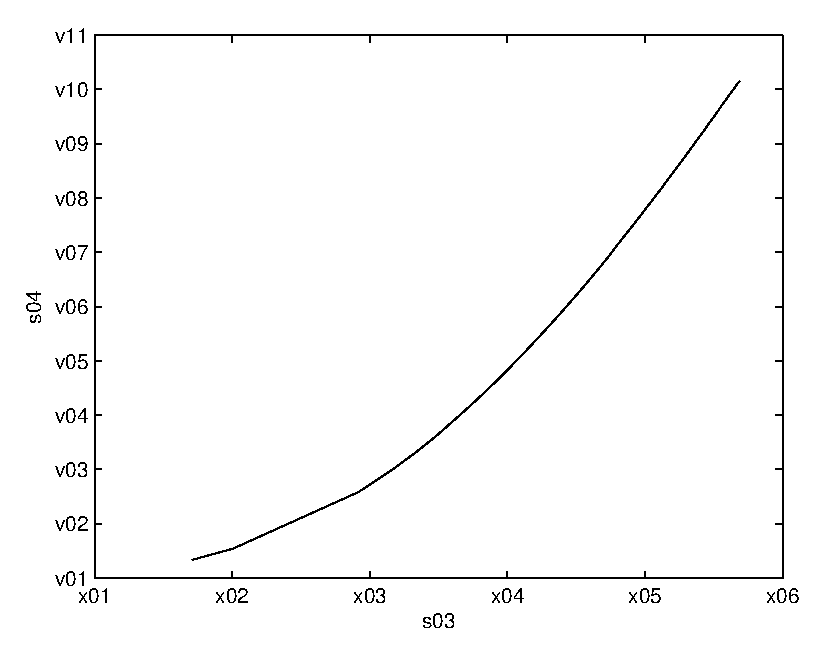
\includegraphics{N_ratio.eps}}%
\end{psfrags}%
%
% End N_ratio.tex
\end{document}
% See http://www.mathworks.de/matlabcentral/fileexchange/loadFile.do?objectId=4638
% for recent versions of laprint.m.
%
% created by:           LaPrint version 3.16 (13.9.2004)
% created on:           13-Aug-2010 12:23:46
% eps bounding box:     15 cm x 11.25 cm
% comment:              
%
\begin{psfrags}%
\psfragscanon%
%
% text strings:
\psfrag{s03}[t][t]{\color[rgb]{0,0,0}\setlength{\tabcolsep}{0pt}\begin{tabular}{c}$1/N$\end{tabular}}%
\psfrag{s04}[b][b]{\color[rgb]{0,0,0}\setlength{\tabcolsep}{0pt}\begin{tabular}{c}$E_\text{PM}/E_\text{Martel}$\end{tabular}}%
%
% xticklabels:
\psfrag{x01}[t][t]{0}%
\psfrag{x02}[t][t]{0.2}%
\psfrag{x03}[t][t]{0.4}%
\psfrag{x04}[t][t]{0.6}%
\psfrag{x05}[t][t]{0.8}%
\psfrag{x06}[t][t]{1}%
%
% yticklabels:
\psfrag{v01}[r][r]{0}%
\psfrag{v02}[r][r]{0.1}%
\psfrag{v03}[r][r]{0.2}%
\psfrag{v04}[r][r]{0.3}%
\psfrag{v05}[r][r]{0.4}%
\psfrag{v06}[r][r]{0.5}%
\psfrag{v07}[r][r]{0.6}%
\psfrag{v08}[r][r]{0.7}%
\psfrag{v09}[r][r]{0.8}%
\psfrag{v10}[r][r]{0.9}%
\psfrag{v11}[r][r]{1}%
%
% Figure:
\resizebox{8.5cm}{!}{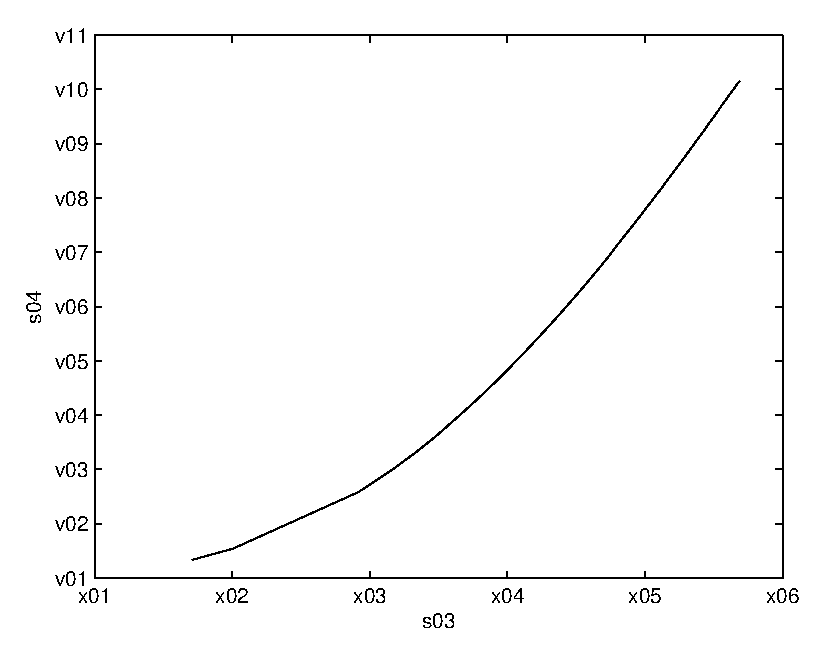
\includegraphics{N_ratio.eps}}%
\end{psfrags}%
%
% End N_ratio.tex
\end{document}
% See http://www.mathworks.de/matlabcentral/fileexchange/loadFile.do?objectId=4638
% for recent versions of laprint.m.
%
% created by:           LaPrint version 3.16 (13.9.2004)
% created on:           13-Aug-2010 12:23:46
% eps bounding box:     15 cm x 11.25 cm
% comment:              
%
\begin{psfrags}%
\psfragscanon%
%
% text strings:
\psfrag{s03}[t][t]{\color[rgb]{0,0,0}\setlength{\tabcolsep}{0pt}\begin{tabular}{c}$1/N$\end{tabular}}%
\psfrag{s04}[b][b]{\color[rgb]{0,0,0}\setlength{\tabcolsep}{0pt}\begin{tabular}{c}$E_\text{PM}/E_\text{Martel}$\end{tabular}}%
%
% xticklabels:
\psfrag{x01}[t][t]{0}%
\psfrag{x02}[t][t]{0.2}%
\psfrag{x03}[t][t]{0.4}%
\psfrag{x04}[t][t]{0.6}%
\psfrag{x05}[t][t]{0.8}%
\psfrag{x06}[t][t]{1}%
%
% yticklabels:
\psfrag{v01}[r][r]{0}%
\psfrag{v02}[r][r]{0.1}%
\psfrag{v03}[r][r]{0.2}%
\psfrag{v04}[r][r]{0.3}%
\psfrag{v05}[r][r]{0.4}%
\psfrag{v06}[r][r]{0.5}%
\psfrag{v07}[r][r]{0.6}%
\psfrag{v08}[r][r]{0.7}%
\psfrag{v09}[r][r]{0.8}%
\psfrag{v10}[r][r]{0.9}%
\psfrag{v11}[r][r]{1}%
%
% Figure:
\resizebox{8.5cm}{!}{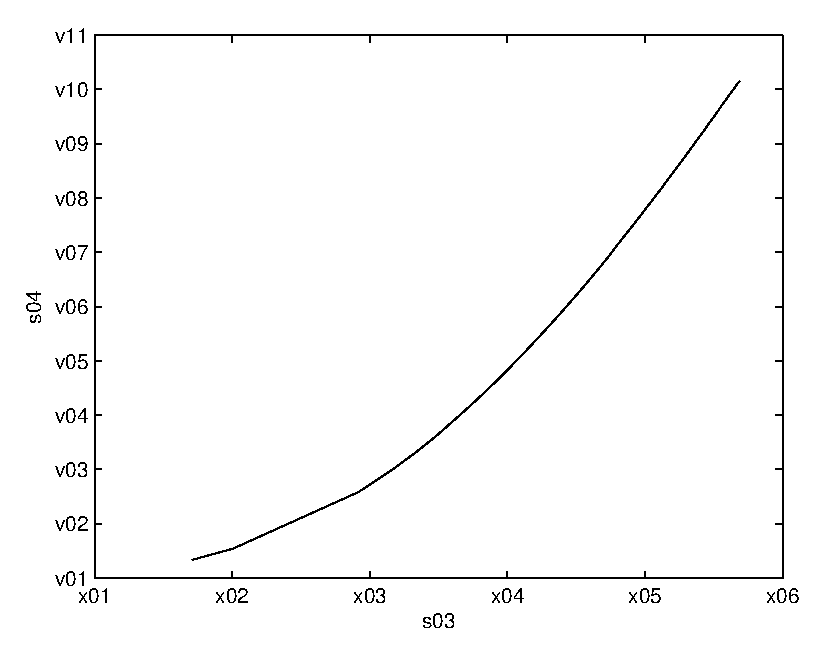
\includegraphics{N_ratio.eps}}%
\end{psfrags}%
%
% End N_ratio.tex
\end{document}
% See http://www.mathworks.de/matlabcentral/fileexchange/loadFile.do?objectId=4638
% for recent versions of laprint.m.
%
% created by:           LaPrint version 3.16 (13.9.2004)
% created on:           13-Aug-2010 12:23:46
% eps bounding box:     15 cm x 11.25 cm
% comment:              
%
\documentclass[11pt]{article}
\usepackage[margin=0, paperwidth=75mm, paperheight=59mm]{geometry}

\usepackage{graphicx,color,psfrag}
\usepackage{amsfonts,amssymb,amsmath}

%\special{papersize=7.5cm,5.9cm}

%% The stock paper size
%\setstocksize{63mm}{79mm}

%% The 'real' page size
%\settrimmedsize{59mm}{75mm}{*}

%% The stock paper will be trimmed 3mm from the
%% top edge and 3mm from the left edge
%\settrims{2mm}{2mm}

%% Spine and trim page margins from main typeblock
%\setlrmarginsandblock{0mm}{0mm}{*}

%% Top and bottom page margins from main typeblock
%\setulmarginsandblock{0mm}{0mm}{*}

%% Header occupies height of a single line;
%% Bottom edge of footer is 7mm from bottom edge
%% of typeblock
%\setheadfoot{\baselineskip}{0mm}

%% Bottom edge of header is 7mm from top edge of
%% typeblock
%\setlength\headsep{0mm}

%% Apply and enforce layout
%\checkandfixthelayout

\begin{document}

\begin{figure}
\centering
\begin{psfrags}%
\psfragscanon%
%
% text strings:
\psfrag{s03}[t][t]{\color[rgb]{0,0,0}\setlength{\tabcolsep}{0pt}\begin{tabular}{c}{\Large$1/N$}\end{tabular}}%
\psfrag{s04}[b][b]{\color[rgb]{0,0,0}\setlength{\tabcolsep}{0pt}\begin{tabular}{c}{\Large$E_\text{PM}/E_\text{Martel}$}\end{tabular}}%
%
% xticklabels:
\psfrag{x01}[t][t]{0}%
\psfrag{x02}[t][t]{0.2}%
\psfrag{x03}[t][t]{0.4}%
\psfrag{x04}[t][t]{0.6}%
\psfrag{x05}[t][t]{0.8}%
\psfrag{x06}[t][t]{1}%
%
% yticklabels:
\psfrag{v01}[r][r]{0}%
\psfrag{v02}[r][r]{0.1}%
\psfrag{v03}[r][r]{0.2}%
\psfrag{v04}[r][r]{0.3}%
\psfrag{v05}[r][r]{0.4}%
\psfrag{v06}[r][r]{0.5}%
\psfrag{v07}[r][r]{0.6}%
\psfrag{v08}[r][r]{0.7}%
\psfrag{v09}[r][r]{0.8}%
\psfrag{v10}[r][r]{0.9}%
\psfrag{v11}[r][r]{1}%
%
% Figure:
\resizebox{7.5cm}{!}{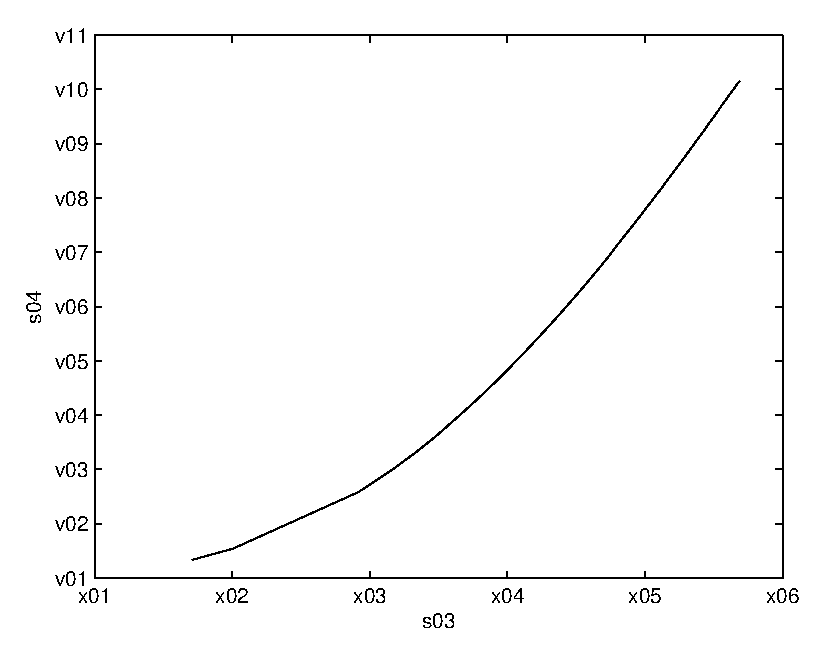
\includegraphics{N_ratio.eps}}%
\end{psfrags}%
%
% End N_ratio.tex
\end{figure}

\end{document}
